
\section{Theorie}
\label{sec:Theorie}

%\subsection{Das Emissionsspektrum von Röntgenstrahlung}

Röntgenstrahlung kann mit einer Röntgenröhre erzeugt werden. Hier werden Elektronen in einer Vakuumröhre aus einer Glühkathode emittiert und mit einer Beschleunigungsspannung $U_.B$ zur Anode hin beschleunigt. 
Beim Auftreffen auf die Anode werden die Elektronen durch das Coulombfeld der Atomkerne abgebremst und der Energieverlust der Elektronen wird in Form von Röntgenstrahlung freigesetzt. Diese Röntgenstrahlung wird als Bremsstrahlung bezeichnet. Bei dem entstehendem Bremsspektrum handelt es sich um ein kontinuierliches Spektrum, da das Elektron entweder nur einen Teil, oder seine gesamte kinetische Energie abgeben kann.\\
Die maximale Energie und damit die minimale Wellenlänge $\lambda_.{min}$ der Röntgenstrahlung ergibt sich also aus der maximalen kinetischen Energie der emittierten Elektronen:
\begin{equation}
\lambda_.{min} = \frac{hc}{E_.{kin,max}} = \frac{hc}{e_0U_.B}\text{.}\label{eq:lambda_min}
\end{equation}
Dabei entspricht $e_0$ der Elementarladung des Elektrons.
Neben der Bremsstrahlung entsteht zusätzlich noch die charakteristische Strahlung. Diese ist vom Anodenmaterial abhängig und entsteht, wenn durch die einfallenden Elektronen die Atome des Anodenmaterials so ionisiert werden, dass ein Elektron aus einer inneren Schale des Atoms gestoßen wird, sodass Elektronenlöcher entstehen.\\
Fällt ein Elektron aus einer höheren Schale an die nun freie Stelle in der inneren Schale zurück, so wird die Energiedifferenz $\Delta E$ der Energieniveaus als Röntgenstrahlung freigesetzt. Da die Energiedifferenz ein fester Wert ist, besteht das charakteristische Röntgenspektrum aus scharfen Linien. Je nachdem in welche Schale das Elektron zurückfällt und von wo es kommt, entstehen demnach unterschiedliche Röntgenlinien. Diese werden $K_\alpha$-, $K_\beta$-, $L_\alpha$-, \dots Linien genannt.\\
Da die Elektronen des Atoms die Kernladung abschirmen, wird zur Berechnung der Bindungsenergie $E_n$ eines Elektrons auf der $n$-ten Schale eine effektive Kernladung $Z_.{eff} = Z-\sigma_n$ eingeführt:
\begin{equation}
E_n = -R_\infty\frac{Z_.{eff}^2}{n^2}\text{.}\label{eq:E_n}
\end{equation}  
Dabei entspricht $R_\infty$ der Rydbergenergie und $\sigma_n$ ist die Abschirmkonstante, welche sich für jedes Elektron unterscheidet. 
Aufgrund von dem Bahndrehimpuls und dem Spin der Elektronen ist dabei jede charakteristische Linie noch weiter aufgespalten in eine Fein- und Hyperfeinstruktur. Diese können jedoch nur mit geeigneten Messinstrumenten aufgelöst werden.
Bei der Messung der Röntgenstrahlung erhält man eine Überlagerung der Bremsstrahlung und der charakteristischen Strahlung (vergleiche Abbildung \ref{fig:Emission}).

\begin{figure}
\centering
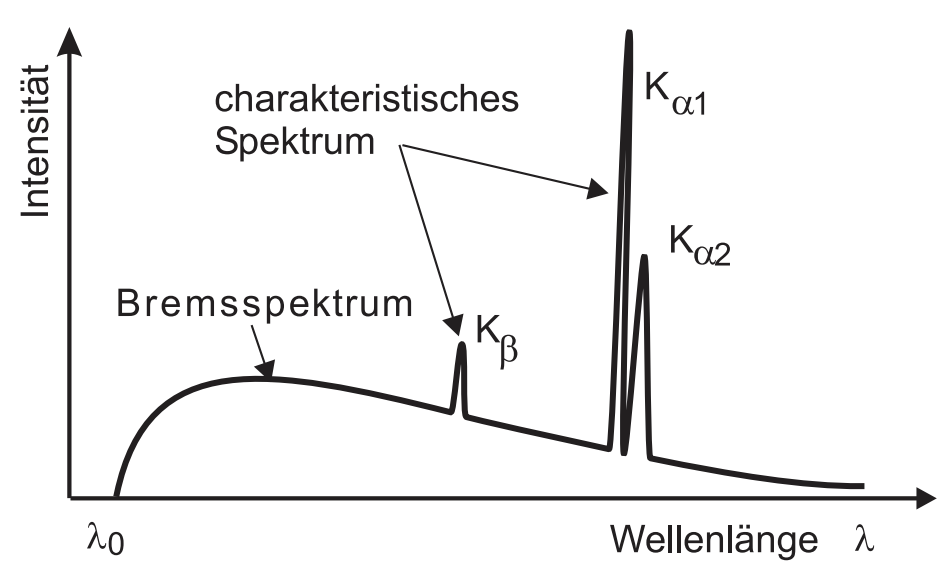
\includegraphics[width=\linewidth-100pt,height=\textheight-100pt,keepaspectratio]{content/images/EmissionsSpektrum.png}
\caption{Beispiel für das Emissionsspektrum einer Röntgenröhre \cite{V602_Emissionsspektrum}.}
\label{fig:Emission}
\end{figure}

%\subsection{Das Absorptionsspektrum von Röntgenstrahlung}

\begin{wrapfigure}[17]{r}{5cm}
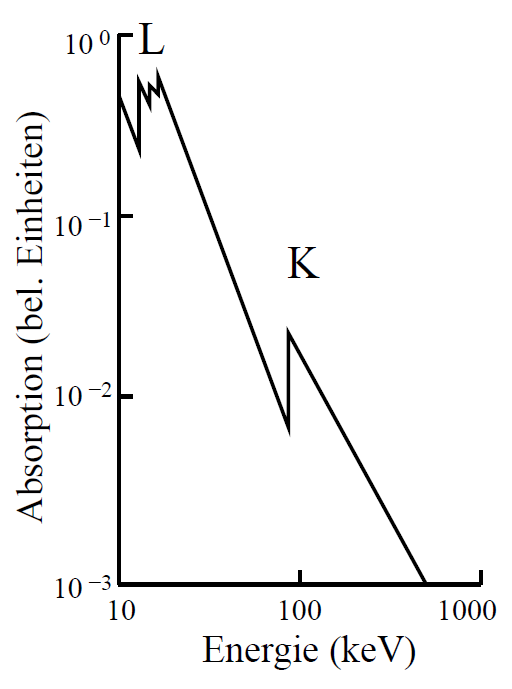
\includegraphics[scale=0.3]{content/images/AbsorptionsSpektrum.png}
\caption{Absorption \cite{V602}.}
\label{fig:Absorption}
\end{wrapfigure}

\noindent Unter einer Energie von $\SI{1}{\mega\electronvolt}$ spielen bei der Absorption von Röntgenstrahlung überwiegend der Comptoneffekt und der Photoeffekt eine Rolle.
Der Absorptionskoeffizient nimmt bei zunehmender Energie ab, besitzt jedoch an den Stellen, wo ein Elektron auf eine höhere Energie angeregt werden kann sogenannte K-, L-, M-, \dots Absorptionskanten (vergleiche Abbildung \ref{fig:Absorption}).\\
Bei der Bestimmung der Bindungsenergie $E_{n,j}$ muss unter Berücksichtigung der Feinstruktur die Sommerfeldsche Feinstrukturformel angewandt werden:
\begin{equation}
E_{n,j} = -R_\infty\left(\frac{Z_.{eff,1}^2}{n^2}+\alpha^2\frac{Z_.{eff,2}}{n^3}\left(\frac{1}{j+\frac{1}{2}}-\frac{3}{4n}\right)\right)\text{.}
\end{equation}
Dabei ist $\alpha$ die Sommerfeldsche Feinstrukturkonstante, $n$ die Hauptquantenzahl und $j$ der Gesamtdrehimpuls des betrachteten Elektrons.
Zur Bestimmung von $\sigma_.L$ der L-Kante, wird die Energiedifferenz $\Delta E_.L$ der L-II- und L-III-Kante betrachtet:
\begin{equation}
\sigma_.L = Z-\sqrt{\left(\frac{4}{\alpha}\sqrt{\frac{\Delta E_.L}{R_\infty}}-\frac{5\Delta E_.L}{R_\infty}\right)\left(1+\frac{19}{32}\alpha^2\frac{\Delta E_.L}{R_\infty}\right)}\text{.}\label{eq:sigma_L}
\end{equation}

\noindent Die Wellenlänge $\lambda$ und somit die Energie der Röntgenstrahlung kann Experimentell über die Bragg-Bedingung bestimmt werden:
\begin{equation}
2d\sin\theta = n\lambda\text{.}\label{eq:Bragg}
\end{equation}
Diese folgt aus der Bragg-Reflexion (Abbildung \ref{fig:Bragg}), bei der die Röntgenstrahlung auf ein dreidimensionales Gitter mit der Gitterkonstanten $d$ fällt. Dort wird sie an jedem Atom gebeugt, sodass bei dem Glanzwinkel $\theta$ konstruktive Interferenz beobachtet werden kann.

\begin{figure}
\centering
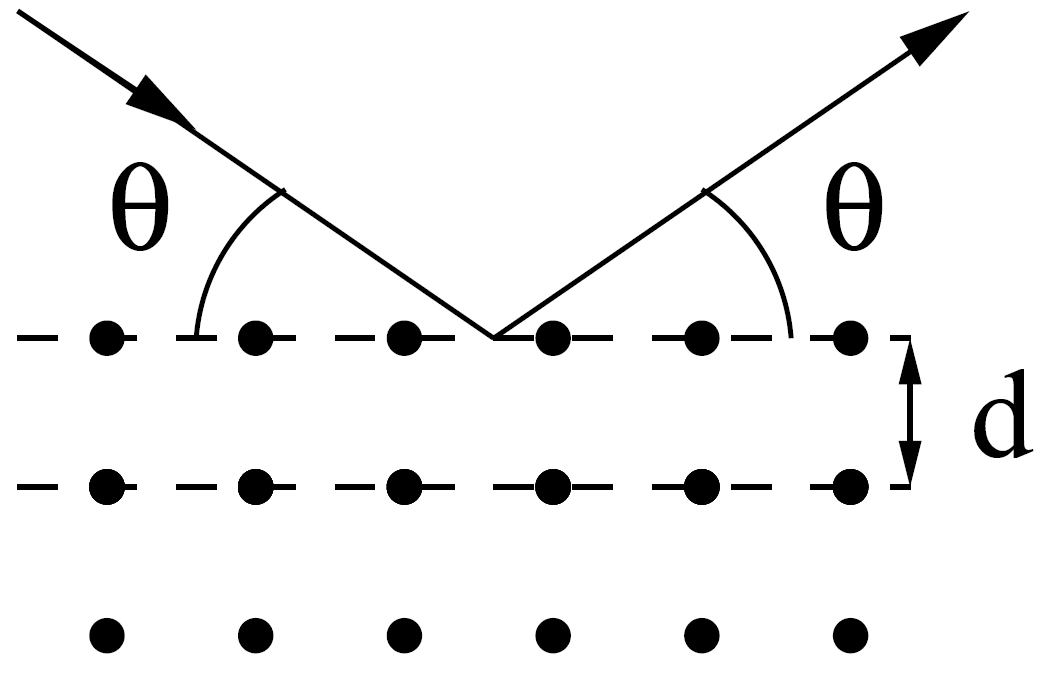
\includegraphics[scale=0.2]{content/images/BraggReflexion.png}
\caption{Skizze zur Bragg-Reflexion \cite{V602}.}
\label{fig:Bragg}
\end{figure}